\documentclass[12pt, openany]{book}
\usepackage[a4paper, margin=1in]{geometry}
\usepackage[utf8]{inputenc}
\usepackage{lmodern}
\usepackage{changepage}
\usepackage{tikz}
\usepackage{tikz-3dplot}
\usetikzlibrary{positioning, fit, arrows.meta, shapes, matrix, shadings}
\usepackage{adjustbox}
\usepackage{amsmath}
\usepackage{caption}
\usepackage{pgfplots}
\usepackage{multirow}
\usepackage{array}
\usepackage{booktabs}
\usepackage[x11names, rgb]{xcolor}
\usepackage{pgfplotstable}
\usepackage{graphicx}
\usepackage{caption}
\usepackage{subcaption}
\usepackage{pgfmath-xfp}
\usepackage{titlesec}
\usepackage{setspace}
\usepackage{tcolorbox}
\usepackage{listings}
\usepackage{tcolorbox}
\usepackage{hyperref}
\usepackage{xparse}

% Required packages
\usepackage{fontspec}
\usepackage{listings}
\usepackage{xcolor}

% Load JetBrains Mono font
\setmonofont{JetBrainsMono}[
    Scale=MatchLowercase,
    Path=./resources/fonts/,
    Extension=.ttf,
    UprightFont=*-Regular,
    BoldFont=*-Bold,
    ItalicFont=*-Italic,
    BoldItalicFont=*-BoldItalic
]

% Define colors
\definecolor{codeblue}{rgb}{0,0,1}
\definecolor{backcolour}{rgb}{0.95,0.95,0.92}
\definecolor{white}{rgb}{1,1,1}
\definecolor{sectionTitleColor}{HTML}{1A73E8}

\definecolor{codeBg}{HTML}{f0f8ff}
\definecolor{codegreen}{rgb}{0,0.6,0}
\definecolor{codegray}{rgb}{0.5,0.5,0.5}
\definecolor{codepurple}{rgb}{0.58,0,0.82}
\definecolor{codeBorder}{HTML}{54b2ff}

% Define colors dark
\definecolor{codeBg}{RGB}{40, 42, 54} 
\definecolor{codegreen}{RGB}{80, 250, 123}  
\definecolor{codegray}{RGB}{248, 248, 242} 
\definecolor{codepurple}{RGB}{189, 147, 249}
\definecolor{codeBorder}{RGB}{98, 114, 164}

\definecolor{codeBlue}{HTML}{38BDF8}

% Define listing style
\lstdefinestyle{mystyle}{
    backgroundcolor=\color{codeBg},   
    commentstyle=\color{codegreen},
    keywordstyle=\color{codeBlue},
    numberstyle=\ttfamily\normalsize\color{codeBg},
    stringstyle=\color{codepurple},
    basicstyle=\ttfamily\normalsize\color{white},
    breakatwhitespace=false,         
    breaklines=true,                 
    captionpos=b,                    
    keepspaces=false,                 
    numbers=left,                    
    numbersep=10pt,                  
    showspaces=false,                
    showstringspaces=false,
    showtabs=false,
    frame=tb,
    rulecolor=\color{codeBg},
    columns=fullflexible,
    aboveskip=10pt,
    belowskip=10pt,
    framesep=10pt,
    lineskip=-0.5pt, % Reduce space between lines
    framerule=0.5pt, % Adjust frame thickness
}

% Apply the style
\lstset{style=mystyle, gobble=3}

\newtcolorbox{roundedlisting}{
    colback=backcolour, % Background color
    colframe=backcolour,  % Border color
    arc=1mm,            % Radius of the rounded corners
    boxrule=0pt,      % Border thickness
    width=\linewidth    % Match the text width
}

\tikzstyle{startstop} = [rectangle, rounded corners, minimum width=3cm, minimum height=1cm,text centered, draw=black, fill=red!30]
\tikzstyle{process} = [rectangle, minimum width=3cm, minimum height=1cm, text centered, draw=black, fill=blue!20]
\tikzstyle{decision} = [diamond, minimum width=3cm, minimum height=1cm, text centered, draw=black, fill=green!20]
\tikzstyle{arrow} = [thick,->,>=stealth]

\newcommand{\code}[1]{\colorbox{gray!20}{\textbf{\texttt{#1}}}}
\ExplSyntaxOn
\NewDocumentCommand{\ui}{m o}
 {
  \group_begin:
  \colorlet{uiback}{gray!20} % Default background
  \colorlet{uiframe}{gray!50} % Default frame
  \colorlet{uitext}{black}    % Default text color
  \IfValueT{#2}
   {
    \str_case:nnF {#2}
     {
      {w} % Warning (yellow)
       {
        \colorlet{uiback}{yellow!20}
        \colorlet{uiframe}{yellow!50}
        \colorlet{uitext}{yellow!70} % Match text color to frame
       }
      {d} % Danger (red)
       {
        \colorlet{uiback}{red!20}
        \colorlet{uiframe}{red!50}
        \colorlet{uitext}{red!70} % Match text color to frame
       }
      {i} % Info (blue)
       {
        \colorlet{uiback}{blue!20}
        \colorlet{uiframe}{blue!50}
        \colorlet{uitext}{blue!70} % Match text color to frame
       }
     }
     {} % Handle invalid options (do nothing)
   }
  \tcbox[
    on~line,
    colback=uiback,
    colframe=uiframe,
    coltext=uitext, % Set text color
    boxrule=0.3pt,
    arc=3pt,
    left=2pt,
    right=2pt,
    top=1pt,
    bottom=1pt
   ]
   {
    \textbf{\texttt{#1}}
   }
  \group_end:
 }
\ExplSyntaxOff
\newcommand{\warning}[1]{%
    \tcbox[colback=red!5, colframe=red!75, boxrule=0.3pt, arc=3pt, left=2pt, right=2pt, top=1pt, bottom=1pt]{\textbf{#1}}%
}

\newtcolorbox{warningbox}{
    colback=red!5,
    colframe=red!75,
    boxrule=0.3pt,
    arc=3pt,
    left=4pt,
    right=4pt,
    top=2pt,
    bottom=2pt,
    width=\linewidth, % Ensures it doesn't overflow
}

\newtcolorbox{infobox}{
    colback=blue!5,
    colframe=blue!75,
    boxrule=0.3pt,
    arc=3pt,
    left=4pt,
    right=4pt,
    top=2pt,
    bottom=2pt,
    width=\linewidth, % Ensures it doesn't overflow
}

\pagenumbering{roman}

\author{
    \textbf{Galib Jaman}\\
}
\date{August 2024}

\begin{document}

\begin{titlepage}
    \centering
    % University Logo
    
\includegraphics[width=0.15\textwidth]{logo.jpg} % Adjust width as needed

    \vspace{1.5cm}

    % Institution and Department Name in Small Caps
    {\Large \textsc{University of Global Village (UGV), Barishal}} \\[0.3cm]
    {\large \textsc{Department of Computer Science and Engineering}} \\[0.5cm]

    \vspace{2cm}

    % Main Title in Huge Bold Font
    {\Huge \textbf{C Programming Guide Book} \par}

    \vspace{2.5cm}

    % Author Name
    {\large \textbf{By} \par}
    \vspace{1cm}
    {\large \textbf{Galib Jaman} \par}
    \vspace{10pt}
    {\normalsize Lab Instructor \par}
    {\normalsize Department of Computer Science and Engineering \par}

    \vfill % Pushes the date to the bottom

    % Date
    {\Large February 2025}
\end{titlepage}


\onehalfspacing
\tableofcontents
% \addcontentsline{toc}{chapter}{List of Tables}

\titleformat{\section}{\normalsize\bfseries}{\thesection}{1em}{}
\titleformat{\subsection}{\normalsize\bfseries}{\thesubsection}{1em}{}

\titleformat{\section}
  {\color{sectionTitleColor}\normalfont\large\bfseries} % Change "blue" to your preferred color
  {\thesection}{1em}{}


  \chapter{Introduction to C Programming}
  \pagenumbering{arabic}
  Let's think about a simple question. How does a computer understand anything? How does a computer differentiate between a number and a character? The simple answer is it doesn't. Then, how does it work? To answer this simple concept we've to first understand the fundamental building blocks of a computer. Electric circuits!
  
  \noindent Now, let's think about a simple electric circuit. It doesn't understand numbers or characters either. But what it does understand is the presence or absence of electricity. If there is electricity, it's a 1. If there is no electricity, it's a 0. That's it! That's the fundamental building block of a computer. It's called a bit. A bit is the smallest unit of data in a computer. It can have only two values, 0 or 1. A group of 8 bits is called a byte. A byte can represent 256 different values (2\textsuperscript{8}).
  
  \noindent That's why every instruction we give to a computer needs to be converted into a series of 0s and 1s. This is called machine language. It's the lowest level of programming languages. Let's take a simple example. Let's say we want to output "Hello, World!" to the screen. In machine language, it would look something like this: 
  \begin{tcolorbox}[colback=lightgray!10, colframe=black, title=Machine Language Code]
      01001000 01100101 01101100 01101100 01101111 00101100 00100000 01010111 01101111 01110010 01101100 01100100 00100001
  \end{tcolorbox}
  \noindent It's not very readable, is it? That's where the programming languages such as C come in.
  
  \section{What is C?}
  C is a general-purpose, procedural computer programming language developed by Dennis Ritchie at Bell Labs in the early 1970s. It was designed to be a small, efficient language that could be used for a wide range of applications. C is a low-level language, which means that it provides a lot of control over the hardware of the computer. This makes it a powerful language, but also more difficult to learn and use than higher-level languages like Python or Java. Let's take a look at a simple "Hello, World!" program written in C:
  \begin{lstlisting}[language=C, caption=Hello World in C]
      #include <stdio.h>
      
      int main() {
          printf("Hello, World!\n");
          return 0;
      }
  \end{lstlisting}
  \noindent This program will output "Hello, World!" to the screen. It's much easier to read and write than the machine language equivalent! Computers don't understand C directly, so we need to compile the C code into machine code before we can run it. This is done using a compiler. The compiler takes the C code as input and produces an executable file that the computer can run.
  
  \section{Installing an IDE and a Compiler}
  To write and run C programs, you need two things: an Integrated Development Environment (IDE) and a C compiler. An IDE is a software application that provides a set of tools for writing, compiling, and debugging code. A C compiler is a program that translates C code into machine code that the computer can run. There are many IDEs and compilers available for C programming. We will be using the Code::Blocks IDE and the GCC compiler in this guide. Here's how you can install them:
  \begin{enumerate}
      \item \textbf{Download Code::Blocks:}
      \begin{itemize}
          \item Go to the official Code::Blocks website: \url{http://www.codeblocks.org/}
          \item Navigate to the ``Downloads" section.
          \item Click on the ``Download the binary release" link.
          \item Choose the appropriate version for your operating system (Windows, macOS, or Linux).
          \item Download the installer that includes the GCC compiler (usually named something like \ui{codeblocks-XX.XXmingw-setup.exe} for Windows).
      \end{itemize}
      \item \textbf{Install Code::Blocks:}
      \begin{itemize}
          \item Run the downloaded installer.
          \item Follow the on-screen instructions to complete the installation.
          \item Make sure to select the option to install the GCC compiler during the installation process.
      \end{itemize}
      \item \textbf{Configure Code::Blocks:}
      \begin{itemize}
          \item Launch Code::Blocks after the installation is complete.
          \item Go to \ui{Settings} \textgreater{} \ui{Compiler}.
          \item Ensure that the selected compiler is "GNU GCC Compiler".
          \item Click on \ui{OK} to save the settings.
      \end{itemize}
      \item \textbf{Create a .c File:}
      \begin{itemize}
          \item Go to \ui{File} \textgreater{} \ui{New} \textgreater{} \ui{Empty File}.
          \item Go to \ui{File} \textgreater{} \ui{Save File As} and save the file with a \ui{.c} extension (e.g., \ui{main.c}).
          \item Save the file in a location where you can easily access it.
      \end{itemize}
      \item \textbf{Write and Run Your First Program:}
      \begin{itemize}
          \item Write your C code in the editor.
          \item Click on the \ui{Build} and \ui{Run} buttons to compile and execute your program.
      \end{itemize}
  \end{enumerate}
  
  \section{Basic Structure of a C Program}
  A C program consists of a series of functions. The main function is the entry point of the program, where the execution begins. Here's the basic structure of a C program:
  \begin{lstlisting}[language=C, caption=Basic Structure of a C Program]
      #include <stdio.h>
      
      int main() {
          printf("Hello, World!\n");
          return 0;
      }
  \end{lstlisting}
  \noindent Let's break down the structure of the program:
  \begin{itemize}
      \item \code{\#include <stdio.h>:} This line includes the standard input/output library, which provides functions like \ui{printf()} and \ui{scanf()} for input and output operations. Take a look at line 4 of the program. We used \ui{printf()} function is to output text to the screen. That's why we need to include the \ui{stdio.h} library. The \code{\#include} directive tells the compiler to include the contents of the specified header file (\ui{stdio.h} in this case) in the program.
      \item \code{int main()\{..\}:} This is the main function of the program. It is the entry point of the program, where the execution begins. The function signature \code{int main()} indicates that the main function returns an integer value. The curly braces \code{\{\}} enclose the body of the function.
      \item \code{return 0:} This statement indicates that the program has executed successfully. The value 0 is returned to the operating system to indicate that the program terminated without errors.
  \end{itemize}
  
  \section{Compiling and Running a C Program}
  Okay, now that we have written our first C program, let's compile and run it. Here's how you can do it using Code::Blocks:
  \begin{enumerate}
      \item \textbf{Build and Run Your Program:}
      \begin{itemize}
          \item Click on the \ui{Build > Build and Run} button to compile and execute your program.
          \item You should see the output "Hello, World!" in the console window.
      \end{itemize}
  \end{enumerate}
  
  \section{Comments in C}
  Comments are used to explain the code and make it more readable. They are ignored by the compiler and do not affect the execution of the program. There are two types of comments in C:
  \begin{itemize}
      \item \textbf{Single-line comments:} Begin with \ui{//} and continue until the end of the line.
      \item \textbf{Multi-line comments:} Begin with \ui{/*} and end with \ui{*/}. They can span multiple lines.
  \end{itemize}
  \clearpage
  Here's an example of how to use comments in C:
  \begin{lstlisting}[language=C, caption=Using Comments in C]
      #include <stdio.h>
      
      int main() {
          // single-line comment
          printf("Hello, World!\n"); // single-line comment
          /*
              This is a multi-line comment
              It can span multiple lines
          */
          return 0;
      }
  \end{lstlisting}
  \begin{infobox}
      Comments are an essential part of programming. They help you and others understand the code better. It's a good practice to add comments to explain the purpose of the code, especially for complex or non-obvious parts of the program.
  \end{infobox}
  
  \section{Excersises and Solutions}
  \textbf{Exercise 1: Write a C program to print "Hello, World!" to the screen.}
  
  \begin{lstlisting}[language=C, caption=Solution to Exercise 1]
      #include <stdio.h>
      
      int main() {
          printf("Hello, World!\n");
          return 0;
      }
  \end{lstlisting}
  \begin{tcolorbox}[colback=lightgray!10, colframe=black, title=Output]
      Hello, World!
  \end{tcolorbox}
  \vspace{10pt}
  \noindent\textbf{Exercise 2: Write a C program to print a square of asterisks (*) to the screen using only one printf statement. The square should be 5x5 in size.}
  
  \begin{lstlisting}[language=C, caption=Solution to Exercise 2]
      #include <stdio.h>
      
      int main() {
          printf("*****\n");
          printf("*****\n");
          printf("*****\n");
          printf("*****\n");
          printf("*****\n");
          return 0;
      }
  \end{lstlisting}
  \begin{tcolorbox}[colback=lightgray!10, colframe=black, title=Output]
      ***** \\
      ***** \\
      ***** \\
      ***** \\
      *****
  \end{tcolorbox}
  
  \begin{infobox}
  The \ui{\textbackslash n} character is used to move the cursor to the next line. By repeating the pattern \ui{"*****\textbackslash n"} five times, we create a 5x5 square of asterisks.
  \end{infobox}
  
  \noindent\textbf{Exercise 3: Write a C program to print a triangle of asterisks (*) to the screen using only one printf statement. The triangle should be 3 lines high.}
  
  \begin{lstlisting}[language=C, caption=Solution to Exercise 3]
      #include <stdio.h>
  
      int main() {
          printf("    *\n");
          printf("   ***\n");
          printf("  *****\n");
          return 0;
      }
  \end{lstlisting}
  \begin{tcolorbox}[colback=lightgray!10, colframe=black, title=Output]
      \makebox[12pt]{ }* \\  
      \makebox[6pt]{ }*** \\  
      *****  
  \end{tcolorbox}
  
  
  \clearpage
  
  \chapter{Data Types and Variables in C}
  Let take a character `A' and a whole number 65. They are not the same thing, right? But in the computer's memory, they are stored as a series of 0s and 1s. For example the character `A' is stored as 01000001 and the number 65 is also stored as 01000001. So, how does the computer know whether it's a character or a number? The answer is \textbf{data types}.
  
  \section{Data Type}
  Data types tell the computer how to interpret the data stored in memory. Which one is `A' and which one is 65 in this case. In C, there are several built-in data types that you can use to declare variables. Let's take a look at some of the common data types in C:
  \begin{itemize}
      \item \textbf{int:} Used to store integer values (whole numbers). For example, 5, -3, 0, etc.
      \item \textbf{float:} Used to store floating-point values (real numbers). For example, 3.14, -0.5, 2.0, etc.
      \item \textbf{double:} Similar to float but with higher precision. Used to store double-precision floating-point values. For example, 3.14159, -0.12345, etc.
      \item \textbf{char:} Any single character enclosed in single quotes. For example, 'A', 'b', '1', etc.
      \item \textbf{bool:} Used to store boolean values (true or false). In C, boolean values are represented as 0 (false) or 1 (true). Although C does not have a built-in boolean data type, you can use the \ui{stdbool.h} header file to define boolean values.
      \item \textbf{void:} Represents an empty data type. It is commonly used as the return type of functions that do not return a value.
  \end{itemize}
  
  \section{Variables}
  Imagine you have a box. You can put anything you want in that box. You can put a number, a character, a string, etc. In programming, a variable is like that box. It's a named storage location in memory where you can store a value. You can think of a variable as a box with a label on it. The label is the variable name, and the value inside the box is the data stored in the variable. Let's take a look at how you can declare variables in C:
  \begin{lstlisting}[language=C, caption=Declaring Variables in C]
      int age; // Declares an integer variable named age
      float height; // Declares a float variable named height
      char grade; // Declares a character variable named grade
  \end{lstlisting}
  \noindent Different data types require different amounts of memory to store the data. For example, an \ui{int} variable requires 4 bytes of memory, a \ui{float} variable requires 4 bytes, and a \ui{char} variable requires 1 byte. The size of a variable depends on the data type and the system architecture (32-bit or 64-bit).
  
  \subsection{Declaration and Initialization}
  When you declare a variable, you are telling the compiler to reserve memory for that variable. You can also initialize the variable with an initial value at the time of declaration. Here's how you can declare and initialize variables in C:
  \begin{lstlisting}[language=C, caption=Declaring and Initializing Variables in C]
      int age = 25;
      float height = 5.8; 
      char grade = 'A';
  \end{lstlisting}
  
  \subsection{Variable Naming Rules}
  When naming variables in C, you need to follow certain rules:
  \begin{itemize}
      \item Variable names must begin with a letter or an underscore.
      \item Variable names can contain letters, digits, and underscores.
      \item Variable names are case-sensitive (e.g., \ui{age}, \ui{Age}, and \ui{AGE} are three different variables).
      \item Variable names cannot be keywords or reserved words (e.g., \ui{int}, \ui{float}, \ui{char}, etc.).
      \item Variable names should be descriptive and meaningful (e.g., \ui{age}, \ui{height}, \ui{grade}, etc.).
  \end{itemize}
  
  Here are some examples of valid and invalid variable names:
  \begin{lstlisting}[language=C, caption=Valid and Invalid Variable Names]
      // Valid variable names
      int age;
      float height;
      char grade;
      int _count;
      float totalAmount;
      
      // Invalid variable names
      int 1age; // Cannot start with a digit
      float height@; // Cannot contain special characters
      char grade%; // Cannot contain special characters
      int total amount; // Cannot contain spaces
  \end{lstlisting}
  
  \noindent One more important thing to remember is values stored in variables can be changed during the execution of the program. For example, you can change the value of the \ui{age} variable from 25 to 30 during the execution of the program like this:
  \begin{lstlisting}[language=C, caption=Changing Variable Values]
      int age = 25; // Declare and initialize the age variable
      age = 30; // Change the value of the age variable
  \end{lstlisting}
  \noindent Notice that we didn't use the \ui{int} keyword when changing the value of the variable. We only need to use the data type when declaring the variable, not when changing its value or using it in expressions.
  
  \subsection{Format Specifiers}
  When you want to print a variable of a specific data type using the \ui{printf()} function or scan a value using the \ui{scanf()} function which we will discuss later, you need to use format specifiers. Format specifiers are placeholders that tell the \ui{printf()} and \ui{scanf()} functions how to interpret the data. For example \ui{\%d} is used for integers. So, if you want to print an integer variable, you need to use the \ui{\%d} format specifier like this:
  \begin{lstlisting}[language=C, caption=Using Format Specifiers]
      int age = 25;
      printf("My age is %d years.\n", age);
  \end{lstlisting}
  \begin{tcolorbox}[colback=lightgray!10, colframe=black, title=Output]
      My age is 25 years.
  \end{tcolorbox}
  \noindent The \ui{\%d} format specifier is used to print integer values. Similarly, you can use other format specifiers for different data types. Heres a table to summarize all the concept we've discussed so far:
  
  \begin{table}[h]
      \centering
      \begin{tabular}{|c|c|c|c|}
          \hline
          \textbf{Data Type} & \textbf{Size (bytes)} & \textbf{Format Specifier} & \textbf{Example} \\
          \hline
          int & 4 & \%d & 25, -3, 0 \\
          \hline
          float & 4 & \%f & 3.14, -0.5, 2.0 \\
          \hline
          double & 8 & \%lf & 3.14159, -0.12345 \\
          \hline
          char & 1 & \%c & `A', `b', `1' \\
          \hline
          bool & 1 & \%d & 0 (false), 1 (true) \\
          \hline
      \end{tabular}
      \caption{Common Data Types in C}
  \end{table}
  
  \section{Constants}
  In addition to variables, you can also use constants in C. Constants are fixed values that do not change during the execution of the program. You can define constants using the \ui{\#define} directive or the \ui{const} keyword. Here's how you can define constants in C:
  \begin{lstlisting}[language=C, caption=Defining Constants in C]
      #define PI 3.14159 // Using #define directive
      const int MAX_VALUE = 100; // Using const keyword
  \end{lstlisting}
  
  Here's a example of how to use both variables and constants in a program:
  \begin{lstlisting}[language=C, caption=Using Variables and Constants in C]
      #include <stdio.h>
      
      #define PI 3.14159
      const int MAX_VALUE = 100;
      
      int main() {
          int radius = 5;
          float area = PI * radius * radius;
          printf("The area of the circle is %f.\n", area);
          return 0;
      }
  \end{lstlisting}
  \begin{tcolorbox}[colback=lightgray!10, colframe=black, title=Output]
      The area of the circle is 78.53975.
  \end{tcolorbox}
  
  \section{Taking User Input using scanf()}
  So far, we have been hardcoding the values of variables in our programs. But what if you want to take input from the user? You can use the \ui{scanf()} function to read input from the user. Here's how you can use the \ui{scanf()} function to read an integer value from the user:
  \begin{lstlisting}[language=C, caption=Reading Integer Input from User]
      #include <stdio.h>
      
      int main() {
          int age;
          printf("Enter your age: ");
          scanf("%d", &age);
          printf("Your age is %d.\n", age);
          return 0;
      }
  \end{lstlisting}
  \begin{tcolorbox}[colback=lightgray!10, colframe=black, title=Output]
      Enter your age: 25 \\
      Your age is 25.
  \end{tcolorbox}
  \noindent The \ui{scanf()} function takes two arguments: the format specifier \ui{\%d} and the address of the variable where the input will be stored using the \ui{\&} operator. The \ui{\&} operator is used to get the memory address of a variable. It is used to pass the address of the variable to the \ui{scanf()} function so that it can store the input value in that memory location.
  \begin{warningbox}
      Don't use the \ui{\&} operator when using the \ui{printf()} function to print the value of a variable. The \ui{\&} operator is only used with the \ui{scanf()} function to read input from the user. If you use the \ui{\&} operator with the \ui{printf()} function, it will print the memory address of the variable, not the value stored in the variable.
  \end{warningbox}
  
  \clearpage
  
  \section{Arithmetic Operators}
  C provides a set of arithmetic operators that you can use to perform mathematical operations on variables. Here are some of the common arithmetic operators in C:
  \begin{itemize}
      \item \textbf{+ (Addition):} Adds two operands.
      \item \textbf{- (Subtraction):} Subtracts the second operand from the first operand.
      \item \textbf{* (Multiplication):} Multiplies two operands.
      \item \textbf{/ (Division):} Divides the first operand by the second operand.
      \item \textbf{\% (Modulus):} Returns the remainder of the division of the first operand by the second operand. For example, $5 \% 2 = 1$.
      \item \textbf{++ (Increment):} Increases the value of the operand by 1.
      \item \textbf{-- (Decrement):} Decreases the value of the operand by 1.
  \end{itemize}
  
  Here's an example of how you can use arithmetic operators in C:
  \begin{lstlisting}[language=C, caption=Using Arithmetic Operators in C]
      #include <stdio.h>
      
      int main() {
          int a = 5, b = 3;
          int sum = a + b;
          int difference = a - b;
          int product = a * b;
          int quotient = a / b;
          int remainder = a % b;
          printf("Sum: %d\n", sum);
          printf("Difference: %d\n", difference);
          printf("Product: %d\n", product);
          printf("Quotient: %d\n", quotient);
          printf("Remainder: %d\n", remainder);
          return 0;
      }
  \end{lstlisting}
      
  \begin{tcolorbox}[colback=lightgray!10, colframe=black, title=Output]
      Sum: 8 \\
      Difference: 2 \\
      Product: 15 \\
      Quotient: 1 \\
      Remainder: 2
  \end{tcolorbox}
  
  \section{Exercises and Solutions}
  \textbf{Exercise 1: Write a program to declare variables of different data types and display their sizes using sizeof().}
  
  \begin{lstlisting}[language=C, caption=Solution to Exercise 1]
      #include <stdio.h>
      
      int main() {
          int a;
          float b;
          char c;
          printf("Size of int: %lu bytes\n", sizeof(a));
          printf("Size of float: %lu bytes\n", sizeof(b));
          printf("Size of char: %lu bytes\n", sizeof(c));
          return 0;
      }
  \end{lstlisting}
  \begin{tcolorbox}[colback=lightgray!10, colframe=black, title=Output]
      Size of int: 4 bytes \\
      Size of float: 4 bytes \\
      Size of char: 1 byte
  \end{tcolorbox}
  \begin{infobox}
  The \ui{sizeof()} operator is used to determine the size of a variable or data type in bytes. The \ui{\%lu} format specifier is used to print the size of the variable as an unsigned long integer.
  \end{infobox}
  
  \vspace{10pt}
  \clearpage
  \noindent\textbf{Exercise 2: Write a program to calculate the area of a rectangle. Take the value of length and width from the user}
  
  \begin{lstlisting}[language=C, caption=Solution to Exercise 2]
      #include <stdio.h>
      
      int main() {
          float length, width, area;
          printf("Enter the length of the rectangle: ");
          scanf("%f", &length);
          printf("Enter the width of the rectangle: ");
          scanf("%f", &width);
          area = length * width;
          printf("The area of the rectangle is %0.2f.\n", area);
          return 0;
      }
  \end{lstlisting}
  \begin{tcolorbox}[colback=lightgray!10, colframe=black, title=Output]
      Enter the length of the rectangle: 5 \\
      Enter the width of the rectangle: 3 \\
      The area of the rectangle is 15.00.
  \end{tcolorbox}
  
  \begin{infobox}
      We can declare multiple variables of the same data type in a single line by separating them with commas. For example, \ui{int a, b, c;} declares three integer variables \ui{a}, \ui{b}, and \ui{c}. Similarly, we can declare and initialize variables of the same data type in a single line like this: \ui{int a = 5, b = 10, c = 15;}.
  \end{infobox}
  \begin{infobox}
      The \ui{\%0.2f} format specifier is used to print the floating-point value with two decimal places. If you want to print the value with three decimal places, you can use the \ui{\%0.3f} format specifier and so on.
  \end{infobox}
  
  \clearpage
  \noindent\textbf{Exercise 3: Write a program to convert temperature from Celsius to Fahrenheit. Take the temperature in Celsius from the user and display the temperature in Fahrenheit. The formula to convert temperature from Celsius to Fahrenheit is: $F = \frac{9}{5} \times C + 32$}
  
  \begin{lstlisting}[language=C, caption=Solution to Exercise 3]
      #include <stdio.h>
      
      int main() {
          float celsius, fahrenheit;
          printf("Enter the temperature in Celsius: ");
          scanf("%f", &celsius);
          fahrenheit = (9.0 / 5.0) * celsius + 32;
          printf("The temperature in Fahrenheit is %0.2f.\n", fahrenheit);
          return 0;
      }
  \end{lstlisting}
  \begin{tcolorbox}[colback=lightgray!10, colframe=black, title=Output]
      Enter the temperature in Celsius: 25 \\
      The temperature in Fahrenheit is 77.00.
  \end{tcolorbox}
  \vspace{10pt}
  \noindent\textbf{Exercise 4: Write a program to calculate the area of a circle. Take the radius of the circle from the user. Use constant PI with a value of 3.14159. The formula to calculate the area of a circle is: $A = \pi \times r^2$}
  
  \begin{lstlisting}[language=C, caption=Solution to Exercise 4]
      #include <stdio.h>
      
      #define PI 3.14159
      
      int main() {
          float radius, area;
          printf("Enter the radius of the circle: ");
          scanf("%f", &radius);
          area = PI * radius * radius;
          printf("The area of the circle is %0.2f.\n", area);
          return 0;
      }
  \end{lstlisting}
  \begin{tcolorbox}[colback=lightgray!10, colframe=black, title=Output]
      Enter the radius of the circle: 5 \\
      The area of the circle is 78.54.
  \end{tcolorbox}
  \vspace{10pt}
  \noindent\textbf{Exercise 5: Write a C program to convert specified days into years, weeks and days. Hint: 1 year = 365 days, 1 week = 7 days.}
  
  \begin{lstlisting}[language=C, caption=Solution to Exercise 5]
      #include <stdio.h>
      
      int main() {
          int days, years, weeks, remainingDays;
          printf("Enter the number of days: ");
          scanf("%d", &days);
          years = days / 365;
          weeks = (days % 365) / 7;
          remainingDays = (days % 365) % 7;
          printf("Years: %d\n", years);
          printf("Weeks: %d\n", weeks);
          printf("Days: %d\n", remainingDays);
          return 0;
      }
  \end{lstlisting}
  \begin{tcolorbox}[colback=lightgray!10, colframe=black, title=Output]
      Enter the number of days: 3659 \\
      Years: 10 \\
      Weeks: 1 \\
      Days: 2
  \end{tcolorbox}
  
  \chapter{Conditional Statements in C}
  Conditional statements allow you to make decisions in your program based on certain conditions. You can use conditional statements to execute different blocks of code depending on whether a condition is true or false. In C, you can use the \ui{if}, \ui{else}, and \ui{else if} statements to implement conditional logic.
  
  \section{Comparison Operators}
  Comparison operators are used to compare two values and determine the relationship between them. Here are some common comparison operators in C:
  \begin{itemize}
      \item \textbf{== (Equal to):} Checks if two values are equal.
      \item \textbf{!= (Not equal to):} Checks if two values are not equal.
      \item \textbf{> (Greater than):} Checks if the left operand is greater than the right operand.
      \item \textbf{< (Less than):} Checks if the left operand is less than the right operand.
      \item \textbf{>= (Greater than or equal to):} Checks if the left operand is greater than or equal to the right operand.
      \item \textbf{<= (Less than or equal to):} Checks if the left operand is less than or equal to the right operand.
  \end{itemize}
  
  \section{Logical Operators}
  Logical operators are used to combine multiple conditions in a conditional statement. Here are some common logical operators in C:
  \begin{itemize}
      \item \textbf{\&\& (Logical AND):} Returns true if both conditions are true.
      \item \textbf{|| (Logical OR):} Returns true if at least one condition is true.
      \item \textbf{! (Logical NOT):} Returns true if the condition is false.
  \end{itemize}
  
  \section{If Statement}
  The \ui{if} statement is used to execute a block of code if a condition is true. Here's the syntax of the \ui{if} statement in C:
  \begin{lstlisting}[language=C, caption=If Statement Syntax]
      if (condition) {
          // Code to be executed if the condition is true
      }
  \end{lstlisting}
  
  Here's an example of how you can use the \ui{if} statement in C:
  \begin{lstlisting}[language=C, caption=Using If Statement in C]
      #include <stdio.h>
      
      int main() {
          int age = 25;
          if (age >= 18) {
              printf("You are an adult.\n");
          }
          return 0;
      }
  \end{lstlisting}
  \begin{tcolorbox}[colback=lightgray!10, colframe=black, title=Output]
      You are an adult.
  \end{tcolorbox}
  
  \subsection{Else Statement}
  The \ui{else} statement is used to execute a block of code if the condition in the \ui{if} statement is false. Here's the syntax of the \ui{else} statement in C:
  \begin{lstlisting}[language=C, caption=Else Statement Syntax]
      if (condition) {
          // Code to be executed if the condition is true
      } else {
          // Code to be executed if the condition is false
      }
  \end{lstlisting}
  
  Here's an example of how you can use the \ui{else} statement in C:
  \begin{lstlisting}[language=C, caption=Using Else Statement in C]
      #include <stdio.h>
      
      int main() {
          int age = 15;
          if (age >= 18) {
              printf("You are an adult.\n");
          } else {
              printf("You are a minor.\n");
          }
          return 0;
      }
  \end{lstlisting}
  \begin{tcolorbox}[colback=lightgray!10, colframe=black, title=Output]
      You are a minor.
  \end{tcolorbox}
  
  \begin{infobox}
      The \ui{else} statement is optional but must be used with an \ui{if} or \ui{else if} statement. It cannot be used on its own.
  \end{infobox}
  
  \subsection{Else If Statement}
  The \ui{else if} statement is used to execute a block of code if the condition in the \ui{if} statement is false and another condition is true. You can use multiple \ui{else if} statements to check for multiple conditions. Here's the syntax of the \ui{else if} statement in C:
  \begin{lstlisting}[language=C, caption=Else If Statement Syntax]
      if (condition1) {
          // Code to be executed if condition1 is true
      } else if (condition2) {
          // Code to be executed if condition2 is true
      } else {
          // Code to be executed if all conditions are false
      }
  \end{lstlisting}
  
  Here's an example of how you can use the \ui{else if} statement in C:
  \begin{lstlisting}[language=C, caption=Using Else If Statement in C]
      #include <stdio.h>
      
      int main() {
          int age = 15;
          if (age >= 18) {
              printf("You are an adult.\n");
          } else if (age >= 13) {
              printf("You are a teenager.\n");
          } else {
              printf("You are a child.\n");
          }
          return 0;
      }
  \end{lstlisting}
  \begin{tcolorbox}[colback=lightgray!10, colframe=black, title=Output]
      You are a teenager.
  \end{tcolorbox}
  
  \begin{infobox}
      The \ui{else if} statement must be used after an \ui{if} statement and before an \ui{else} statement. You can have multiple \ui{else if} statements to check for different conditions.
  \end{infobox}
  
  \section{Switch Statement}
  The \ui{switch} statement is used to execute different blocks of code based on the value of an expression. It is an alternative to using multiple \ui{if} statements with \ui{else if} statements. Here's an example of how you can use the \ui{switch} statement in C:
  \begin{lstlisting}[language=C, caption=Using Switch Statement in C]
      #include <stdio.h>
      
      int main() {
          char grade = 'B';
          switch (grade) {
              case 'A':
                  printf("Excellent!\n");
                  break;
              case 'B':
                  printf("Good!\n");
                  break;
              case 'C':
                  printf("Average!\n");
                  break;
              case 'D':
                  printf("Poor!\n");
                  break;
              default:
                  printf("Invalid grade!\n");
          }
          return 0;
      }
  \end{lstlisting}
  \begin{tcolorbox}[colback=lightgray!10, colframe=black, title=Output]
      Good!
  \end{tcolorbox}
  
  \begin{infobox}
      The \ui{break} statement is used to exit the \ui{switch} statement after executing the code block for a particular case. If you omit the \ui{break} statement, the code will continue to execute the code blocks for subsequent cases until it reaches a \ui{break} statement or the end of the \ui{switch} statement.
  \end{infobox}
  
  \subsection{Why Use Switch Statement?}
  The \ui{switch} statement is useful when you have multiple conditions to check against a single expression. It is more concise and easier to read than using multiple \ui{if} statements with \ui{else if} statements. The \ui{switch} statement is also more efficient than using multiple \ui{if} statements because the compiler can optimize the code better.
  
  \section{Exercises and Solutions}
  \textbf{Exercise 1: Write a program to check if a number is positive, negative, or zero. Take the number from the user.}
  
  \begin{lstlisting}[language=C, caption=Solution to Exercise 1]
      #include <stdio.h>
      
      int main() {
          int number;
          printf("Enter a number: ");
          scanf("%d", &number);
          if (number > 0) {
              printf("The number is positive.\n");
          } else if (number < 0) {
              printf("The number is negative.\n");
          } else {
              printf("The number is zero.\n");
          }
          return 0;
      }
  \end{lstlisting}
  \begin{tcolorbox}[colback=lightgray!10, colframe=black, title=Output]
      Enter a number: -5 \\
      The number is negative.
  \end{tcolorbox}
  \vspace{10pt}
  \noindent\textbf{Exercise 2: Write a C program to find whether a given year is a leap year or not. Take the year from the user. A leap year is a year that is divisible by 4 but not divisible by 100, except for years that are divisible by 400.}
  
  \begin{lstlisting}[language=C, caption=Solution to Exercise 2]
      #include <stdio.h>
      
      int main() {
          int year;
          printf("Enter a year: ");
          scanf("%d", &year);
          if ((year % 4 == 0 && year % 100 != 0) || year % 400 == 0) {
              printf("%d is a leap year.\n", year);
          } else {
              printf("%d is not a leap year.\n", year);
          }
          return 0;
      }
  \end{lstlisting}
  \begin{tcolorbox}[colback=lightgray!10, colframe=black, title=Output]
      Enter a year: 2020 \\
      2020 is a leap year.
  \end{tcolorbox}
  \vspace{10pt}
  \noindent\textbf{Exercise 3: Write a program to find the largest of three numbers. Take the numbers from the user.}
  
  \begin{lstlisting}[language=C, caption=Solution to Exercise 3]
      #include <stdio.h>
      
      int main() {
          int num1, num2, num3;
          printf("Enter three numbers: ");
          scanf("%d %d %d", &num1, &num2, &num3);
          if (num1 >= num2 && num1 >= num3) {
              printf("%d is the largest number.\n", num1);
          } else if (num2 >= num1 && num2 >= num3) {
              printf("%d is the largest number.\n", num2);
          } else {
              printf("%d is the largest number.\n", num3);
          }
          return 0;
      }
  \end{lstlisting}
  \begin{tcolorbox}[colback=lightgray!10, colframe=black, title=Output]
      Enter three numbers: 5 10 3 \\
      10 is the largest number.
  \end{tcolorbox}
  \noindent\textbf{Exercise 4: Write a C program to accept a coordinate point in an XY coordinate system and determine in which quadrant the coordinate point lies. Take the values of X and Y from the user.}
  
  \begin{lstlisting}[language=C, caption=Solution to Exercise 4]
      #include <stdio.h>
      
      int main() {
          int x, y;
          printf("Enter the values of X and Y: ");
          scanf("%d %d", &x, &y);
          if (x > 0 && y > 0) {
              printf("First quadrant.\n", x, y);
          } else if (x < 0 && y > 0) {
              printf("Second quadrant.\n", x, y);
          } else if (x < 0 && y < 0) {
              printf("Third quadrant.\n", x, y);
          } else if (x > 0 && y < 0) {
              printf("Fourth quadrant.\n", x, y);
          } else {
              printf("The point (%d, %d) lies on the origin.\n", x, y);
          }
          return 0;
      }
  \end{lstlisting}
  \begin{tcolorbox}[colback=lightgray!10, colframe=black, title=Output]
      Enter the values of X and Y: 5 -3 \\
      The point (5, -3) lies in the fourth quadrant.
  \end{tcolorbox}
  \vspace{10pt}
  \noindent\textbf{Exercise 5: Write a C program to check whether a triangle can be formed with the given values for the angles/sides. To form a triangle, the sum of any two sides must be greater than the third side. Take the lengths of the three sides from the user.}
  
  \begin{lstlisting}[language=C, caption=Solution to Exercise 5]
      #include <stdio.h>
      
      int main() {
          int side1, side2, side3;
          printf("Enter the lengths of the three sides: ");
          scanf("%d %d %d", &side1, &side2, &side3);
          if (side1 + side2 > side3 && side2 + side3 > side1 && side1 + side3 > side2) {
              printf("A triangle can be formed.\n");
          } else {
              printf("A triangle cannot be formed.\n");
          }
          return 0;
      }
  \end{lstlisting}
  \begin{tcolorbox}[colback=lightgray!10, colframe=black, title=Output]
      Enter the lengths of the three sides: 5 10 15 \\
      A triangle cannot be formed.
  \end{tcolorbox}
  \vspace{10pt}
  \noindent\textbf{Exercise 6: Write a C program to check whether a character is an alphabet, digit or special character. Take the character from the user.}
  
  \begin{lstlisting}[language=C, caption=Solution to Exercise 6]
      #include <stdio.h>
      
      int main() {
          char ch;
          printf("Enter a character: ");
          scanf("%c", &ch);
          if ((ch >= 'a' && ch <= 'z') || (ch >= 'A' && ch <= 'Z')) {
              printf("%c is an alphabet.\n", ch);
          } else if (ch >= '0' && ch <= '9') {
              printf("%c is a digit.\n", ch);
          } else {
              printf("%c is a special character.\n", ch);
          }
          return 0;
      }
  \end{lstlisting}
  \begin{tcolorbox}[colback=lightgray!10, colframe=black, title=Output]
      Enter a character: 5 \\
      5 is a digit.
  \end{tcolorbox}

\chapter{Loops and Iteration in C}
Suppose you want to print the numbers from 1 to 5. You can do this by writing five \ui{printf()} statements like this:
\vspace{10pt}
\begin{lstlisting}[language=C, gobble=0]
    printf("1\n");
    printf("2\n");
    printf("3\n");
    printf("4\n");
    printf("5\n");
\end{lstlisting}
\begin{tcolorbox}[colback=lightgray!10, colframe=black, title=Output]
    1 \\
    2 \\
    3 \\
    4 \\
    5
\end{tcolorbox}
\vspace{10pt}
It's one way of doing it. But what if you want to print the numbers from 1 to 100? or 1 to 1000? Writing that many \ui{printf()} statements would be hard to say the least. This is where loops enters the picture like a superhero. Loops allow you to execute a block of code multiple times. Every loop has three main components:
\begin{itemize}
    \item \textbf{Strating Point:} The starting point of the loop.
    \item \textbf{Ending Condition:} The condition that is checked before each iteration of the loop.
    \item \textbf{Increment/Decrement:} The value by which the loop variable is incremented or decremented after each iteration.
\end{itemize}

\clearpage
\noindent \textbf{Here's a flow chart of how a loop works:}
\begin{figure}[h]
\centering
    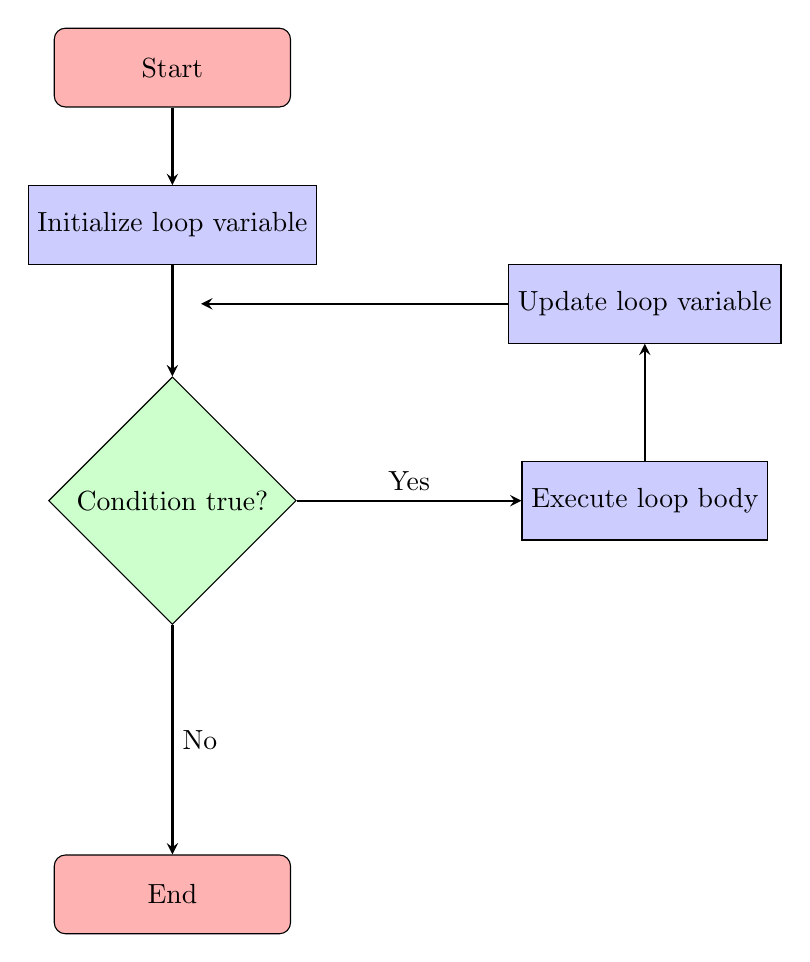
\begin{tikzpicture}[node distance=2cm]
    
        % Nodes
        \node (start) [startstop] {Start};
        \node (init) [process, below of=start] {Initialize loop variable};
        \node (condition) [decision, below of=init, yshift=-1.5cm] {Condition true?};
        \node (process) [process, right of=condition, xshift=4cm] {Execute loop body};
        \node (update) [process, above of=process, yshift=0.5cm] {Update loop variable};
        \node (end) [startstop, below of=condition, yshift=-3cm] {End};
    
        % Arrows
        \draw [arrow] (start) -- (init);
        \draw [arrow] (init) -- (condition);
        \draw [arrow] (condition.east) -- (process.west) node[midway, above] {Yes};
        \draw [arrow] (process) -- (update);
        \draw [arrow] (update.west) -- ++(-3.9cm,0);
        \draw [arrow] (condition.south) -- (end) node[midway, right] {No};
    
    \end{tikzpicture}
    \caption{Flow chart of a loop}
    \vspace{2cm}
    \label{fig:loop_flowchart}
\end{figure}

\section{While Loop}
The \ui{while} loop is used to execute a block of code as long as a condition is true. Here's the syntax of the \ui{while} loop in C:
\begin{lstlisting}[language=C, gobble=0, caption=While Loop Syntax]
    while (condition) {
        // Code to be executed
    }
\end{lstlisting}

\clearpage
\noindent Here's an example of how you can use the \ui{while} loop in C to print the numbers from 1 to 5:
\begin{lstlisting}[language=C, gobble=0, caption=Using While Loop in C]
    #include <stdio.h>
    
    int main() {
        int i = 1; // Part 1: Starting Point
        while (i <= 5) // Part 2: Ending Condition
        { 
            printf("%d\n", i);
            i++; // Part 3: Increment
        }
        return 0;
    }
\end{lstlisting}
\begin{tcolorbox}[colback=lightgray!10, colframe=black, title=Output]
    1 \\
    2 \\
    3 \\
    4 \\
    5
\end{tcolorbox}

\begin{warningbox}
    Make sure that all the three components of the loop are present in the \ui{while} loop. If you forget to update the loop variable, the loop will run indefinitely and cause an infinite loop.
\end{warningbox}

\subsection{When to Use While Loop?}
The \ui{while} loop is used when you don't know the number of iterations in advance and want to execute a block of code as long as a condition is true. For example, you can use a \ui{while} loop to read input from the user until a specific value is entered. On of the most common use of \ui{while} loop is the \textbf{game loop in game development}.

\section{For Loop}
The \ui{for} loop is used to execute a block of code a specified number of times. It is more concise than the \ui{while} loop when you know the number of iterations in advance. Here's the syntax of the \ui{for} loop in C:
\begin{lstlisting}[language=C, gobble=0, caption=For Loop Syntax]
    for (initialization; condition; update) {
        // Code to be executed
    }
\end{lstlisting}

Here's an example of how you can use the \ui{for} loop in C to print the numbers from 1 to 5:
\begin{lstlisting}[language=C, gobble=0, caption=Using For Loop in C]
    #include <stdio.h>
    
    int main() {
        for (int i = 1; i <= 5; i++) {
            printf("%d\n", i);
        }
        return 0;
    }
\end{lstlisting}
\begin{tcolorbox}[colback=lightgray!10, colframe=black, title=Output]
    1 \\
    2 \\
    3 \\
    4 \\
    5
\end{tcolorbox}
\begin{infobox}
    We can declare the loop variable \ui{int i}[i] in this case, inside the \ui{for} loop itself. This is called a \textbf{local variable} and it is only accessible within the loop.
\end{infobox}
\begin{warningbox}
    Make sure that all the three components of the loop are present in the \ui{for} loop and are separated by semicolons \ui{;} \textbf{\textcolor{red}{not commas}} \ui{,}[d].
\end{warningbox}

\subsection{When to Use For Loop?}
The \ui{for} loop is used when you know the number of iterations in advance and want to execute a block of code a specified number of times. It is more concise than the \ui{while} loop when you know the starting point, ending condition, and increment/decrement value.

\clearpage
\section{Do-While Loop}
The \ui{do-while} loop is similar to the \ui{while} loop, but the condition is checked at the end of the loop. This means that the block of code is executed at least once, even if the condition is false. Here's the syntax of the \ui{do-while} loop in C:
\begin{lstlisting}[language=C, gobble=0, caption=Do-While Loop Syntax]
    do {
        // Code to be executed
    } while (condition);
\end{lstlisting}

\noindent Here's the flow chart of how a \ui{do-while} loop works:
\begin{figure}[h]
\centering
    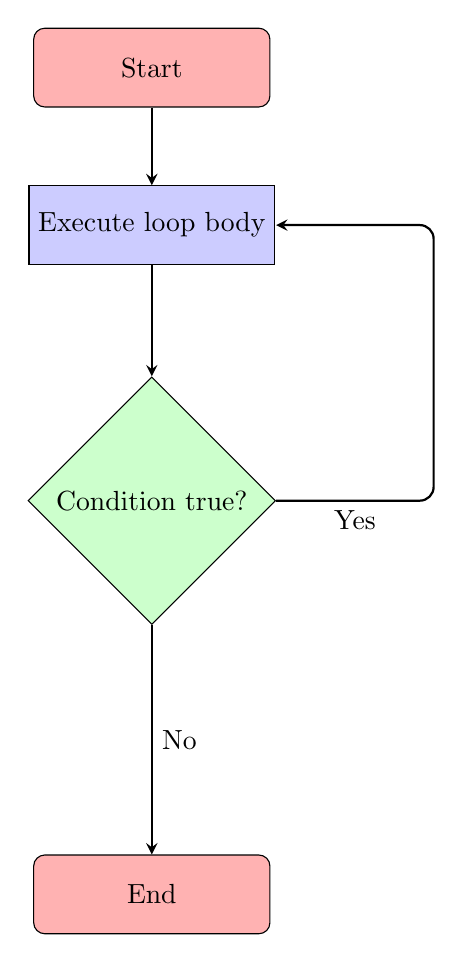
\begin{tikzpicture}[node distance=2cm]
    
        % Nodes
        \node (start) [startstop] {Start};
        \node (process) [process, below of=start] {Execute loop body};
        \node (condition) [decision, below of=process, yshift=-1.5cm] {Condition true?};
        \node (end) [startstop, below of=condition, yshift=-3cm] {End};
    
        % Arrows
        \draw [arrow] (start) -- (process);
        \draw [arrow] (process) -- (condition);
        \draw [arrow, rounded corners=5pt] (condition.east) -- ++(2cm,0)node[midway, below] {Yes} -- ++(0,3.5cm) -- ++(-2cm,0);
        \draw [arrow] (condition.south) -- (end) node[midway, right] {No};
    
    \end{tikzpicture}
    \caption{Flow chart of a do-while loop}
    \vspace{2cm}
    \label{fig:dowhile_flowchart}
\end{figure}

\clearpage
\noindent Here's an example of how you can use the \ui{do-while} loop in C to print the numbers from 1 to 5:
\begin{lstlisting}[language=C, gobble=0, caption=Using Do-While Loop in C]
    #include <stdio.h>
    
    int main() {
        int i = 1;
        do {
            printf("%d ", i);
            i++;
        } while (i <= 5);
        return 0;
    }
\end{lstlisting}
\begin{tcolorbox}[colback=lightgray!10, colframe=black, title=Output]
    1 2 3 4 5
\end{tcolorbox}

\subsection{When to Use Do-While Loop?}
The \ui{do-while} loop is used when you want to execute a block of code at least once, even if the condition is false. It is useful when you want to execute the loop body before checking the condition.

\section{Break and Continue Statements}
The \ui{break} and \ui{continue} statements are used to control the flow of a loop. Here's how they work:
\begin{itemize}
    \item \textbf{Break Statement:} The \ui{break} statement is used to exit the loop immediately. It is used to terminate the loop prematurely.
    \item \textbf{Continue Statement:} The \ui{continue} statement is used to skip the current iteration of the loop and continue with the next iteration. It is used to skip the remaining code in the loop body and move to the next iteration.
\end{itemize}

\clearpage
\noindent Here's an example of how you can use the \ui{break} and \ui{continue} statements in a loop:
\begin{lstlisting}[language=C, gobble=0, caption=Using Break and Continue Statements in C]
    #include <stdio.h>
    
    int main() {
        for (int i = 1; i <= 10; i++) {
            if (i == 3) {
                continue; // Skip the current iteration
            }
            if (i == 5) {
                break; // Exit the loop
            }
            printf("%d ", i);
        }
        return 0;
    }
\end{lstlisting}
\begin{tcolorbox}[colback=lightgray!10, colframe=black, title=Output]
    1 2 4
\end{tcolorbox}

\begin{infobox}
    Notice that the \ui{continue} statement skips the number 3 and the \ui{break} statement exits the loop when the number 5 is encountered even though our stopping condition is \ui{i <= 10}.
\end{infobox}

\section{Nested Loops}
A nested loop is a loop inside another loop. You can use nested loops to perform more complex tasks that require multiple iterations. Here's an example of how you can use nested loops to print a pattern:
\begin{lstlisting}[language=C, gobble=0, caption=Using Nested Loops in C]
    #include <stdio.h>
    
    int main() {
        for (int i = 1; i <= 5; i++) {
            for (int j = 1; j <= i; j++) {
                printf("* ");
            }
            printf("\n");
        }
        return 0;
    }
\end{lstlisting}
\begin{tcolorbox}[colback=lightgray!10, colframe=black, title=Output]
    * \\
    * * \\
    * * * \\
    * * * * \\
    * * * * *
\end{tcolorbox}




\end{document}